\documentclass[a4paper, 9pt]{article}
\usepackage[latin1]{inputenc}
\usepackage[T1]{fontenc}
\usepackage[francais]{babel}
\usepackage{entete}
\usepackage{noitemsep}
\usepackage{euscript} 
\usepackage{amsmath,amssymb,amsfonts,amsthm}
\usepackage{graphicx,graphics,epsfig,subfigure,color}
\usepackage{url}
%\usepackage{algorithm2e}
\usepackage{multicol}
\usepackage{a4wide}
\usepackage{latexsym}
\usepackage{verbatim}
\setlength{\textheight}{24cm}
\setlength{\topmargin}{-0.5cm}
\setlength{\textwidth}{160mm}
\setlength{\oddsidemargin}{1mm}

%\renewcommand{\baselinestretch}{0.85}

%\input{macroAlgo}
%\dontprintsemicolon

\setlength{\parindent}{0pt}  %%suppression indentation


\begin{document}
\selectlanguage{francais}
\author{D. Fourer, L. Lagon}
\newcommand{\universityname}{IUT d'\'Evry Val d'Essonne}
\newcommand{\deptname}{D\'epartement TC (S1)}
\newcommand{\years}{2023-2024}

%------------------- TITRE -----------------------------------------
\date{Septembre 2023} 
\TDHead{\universityname}{\deptname}{R1.13, Ressources et Culture Num\'eriques 1, \years}{\large TD4 : Formulaire / Sondage}
%\TDHead{DUT TC}{}{\large TIC3: Fonctions avanc\'ees d'un tableur}
%-------------------------------------------------------------------
\underline{Objectifs:} Ma\^itrise des outils permettant de r\'ealiser des sondages.
\flushleft
\vspace{-0.2cm}

\section{Formulaire PDF}

%Cette premi\`ere m\'ethode permet de g\'en\'erer des formulaires qui devront par la suite \^etre imprim\'es puis exploit\'es manuellement.

\exost Avec Libreoffice, cr\'eez un nouveau fichier texte. Ajouter le titre ``Questionnaire de satisfaction'' en haut de page centr\'e en utilisant une police Arial de taille 20.

\exost Cr\'eez un formulaire en utilisant les \'el\'ements de contr\^ole disponibles dans le menu ``Formulaire'' en structurant votre document
comme ci-dessous. Vous ajouterez un sous-titre pour chaque rubrique (taille 12):
%
\begin{itemize}
 \item Informations personnelles: 
 \begin{itemize}
  \item Nom (texte)
  \item Pr\'enom (texte)
  \item Date de naissance (date)
  \item Formation (liste parmi FI1/FI2/FA1/FA2)
 \end{itemize}
  \item Cursus suivi: 
  \begin{itemize}
    \item S\'erie BAC (liste parmi g\'en\'eral/techno/pro/autre)
    \item Redoublement (boutons radio permettant de choisir parmi oui et non)
    \item Exp\'erience en entreprise (choix dans une liste parmi aucune/3 mois / 6 mois / entre 1 et 2 ans / plus de 3 ans)
  \end{itemize}
 \item Satisfaction (pour chaque crit\`ere, proposer 4 boutons radios permettant de choisir parmi  tr\`es-bien/assez-bien/moyen/insuffisant/mauvais):
 \begin{itemize}
  \item Qualit\'e des enseignements
  \item Disponibilit\'e des enseignants
  \item \'Etat des Locaux
  \item D\'ebouch\'es offertes par la formation
  \end{itemize}
  \item Traitement des donn\'ees (proposez syst\'ematiquement une simple case \`a cocher):
  \begin{itemize}
    \item Souhaitez-vous recevoir les r\'esultats de ce sondage ?
    \item Accepteriez-vous de participer \`a un nouveau sondage dans quelques mois sur votre devenir professionnel ?
    \item Moyen de communication souhait\'e (plusieurs choix possibles): T\'el\'ephone / e-mail / courrier 
  \end{itemize}
 \end{itemize}

 \exost Enregistrez le document r\'ealis\'e au format odt puis r\'ealisez un export au format PDF. 
 
 \exost Ouvrez le document PDF produit avec un lecteur PDF (eg. Foxit Reader). Activez le formulaire puis assurez-vous que les champs vous proposent bien les options attendues.
 Le cas \'ech\'eant, corrigez votre formulaire pour obtenir un r\'esultat professionnel.

 \underline{Indications:}
 \begin{itemize}
  \item Donnez syst\'ematiquement un nom unique \`a chaque \'el\'ement de votre formulaire (cf. Figure~\ref{fig:prop}) et restreignez les r\'eponses possibles aux seules valeurs autoris\'ees 
  (eg. longueur maximale du texte, valeurs accept\'ees, etc.)
  \item Les boutons radios doivent appartenir au m\^eme groupe pour la m\^eme question et ne doivent autoriser qu'une seule s\'election
  \item Utilisez syst\'ematiquement les \'el\'ements de formulaire correspondants au type de donn\'ees attendues eg. texte, nombre ou date)
 \end{itemize}

 
\section{Formulaire en ligne}
%Cette seconde m\'ethode 

\exost R\'ealisez le m\^eme formulaire via la plate-forme Google Forms\footnote{\url{https://docs.google.com/forms}}. Vous aurez besoin de vous cr\'eer un compte Google
si vous n'en avez pas.

\exost Lancez une invitation \`a un ou plusieurs de vos coll\`egues pour lui demander de compl\'eter le formulaire pour vous.

\exost R\'ealisez un export des r\'eponses obtenues \`a votre formulaire au format CSV. Ouvrez ce fichier et analysez son contenu.

\begin{figure}[ht]
 \centering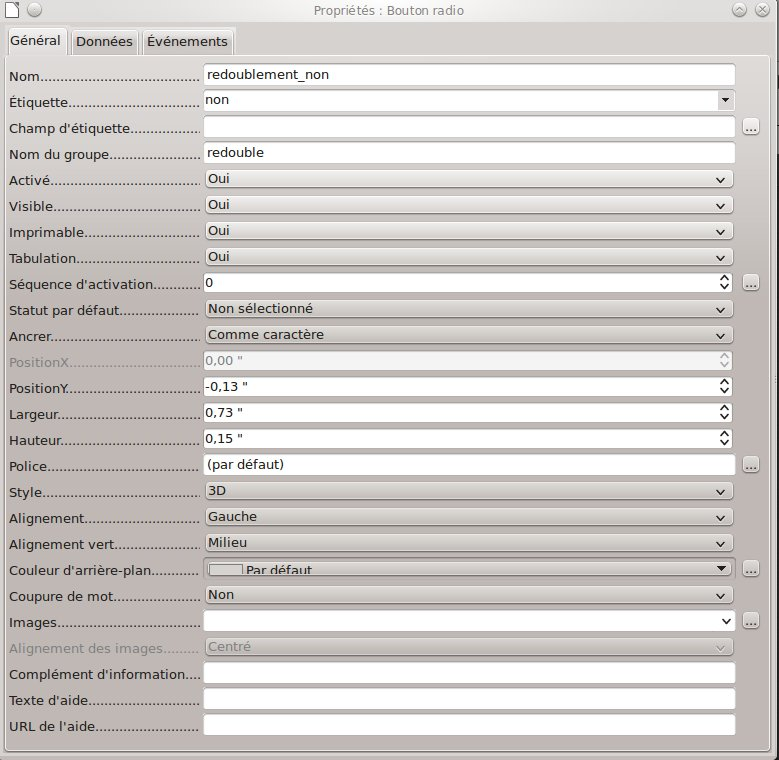
\includegraphics[width=0.7\textwidth]{forms.jpg}
 \caption{Propri\'et\'es d'un \'el\'ement du formulaire.}
 \label{fig:prop}
\end{figure}


% \exost Lancez le logiciel de votre choix (Libreoffice Impress ou PowerPoint) et cr\'eez une pr\'esentation de votre entreprise contenant au minimum 15 diapositives .
% Votre pr\'esentation respectera les consignes suivantes:
% \begin{itemize}
%  \item Votre pr\'esentation respectera le plan suivant :  
%  \begin{itemize}
%   \item Activit\'e
%   \item Organigramme
%   \item analyse SWOT\footnote{forces/faiblesses/opportunit\'es/menaces}
%   \item vos missions
%   \item r\'ealisations
%   \item perspectives
%   \end{itemize}
%  \item Votre pr\'esentation comportera une diapositive de titre comportant votre nom et celle de votre entreprise, ainsi qu'une table des mati\`eres
%  \item Vous int\'egrerez plusieurs images dans votre pr\'esentation, dont le logo de l'IUT et celui de votre entreprise
%  \item Vous ajouterez au minimum 2 transitions diff\'erentes permettant de rendre votre diaporama plus attrayant
%  \item Votre diaporama contiendra au moins une vid\'eo
% \end{itemize}
% 
% \exost Cr\'eez un masque des diapositives original permettant d'obtenir un style personnalis\'e pour votre pr\'esentation.\\
% \centering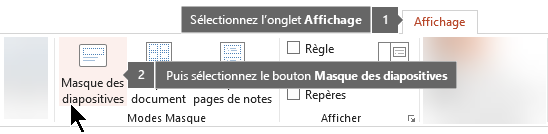
\includegraphics[width=0.8\textwidth]{./masque.png}
% \flushleft
% 
% \exost Ins\'erez la date, l'heure et le num\'ero de chaque diapositive en bas \`a droite de votre pr\'esentation.
% 
% \exost Enregistrez votre pr\'esentations dans les formats suivants: PPTX, PPSX et PDF. Quelle est la diff\'erence entre ces trois formats ?


\end{document}

% End Of File

